\section{Análise de Significância Estatística}

A fim de validar se as diferenças de desempenho observadas entre os modelos são estatisticamente significativas e não fruto do acaso, aplicamos o teste de \textbf{McNemar} pareado. Este teste é ideal para comparar a concordância de erro entre dois classificadores no mesmo conjunto de teste. 

A Figura \ref{fig:p_value_heatmap} apresenta a matriz de calor dos \textit{p-values} para todos os pares de modelos na melhor versão experimental (V10). Os resultados com sufixo (ns) indicam que a diferença entre os modelos não é estatisticamente significativa ($p > 0,05$).

\begin{figure}[h!]
  \centering
  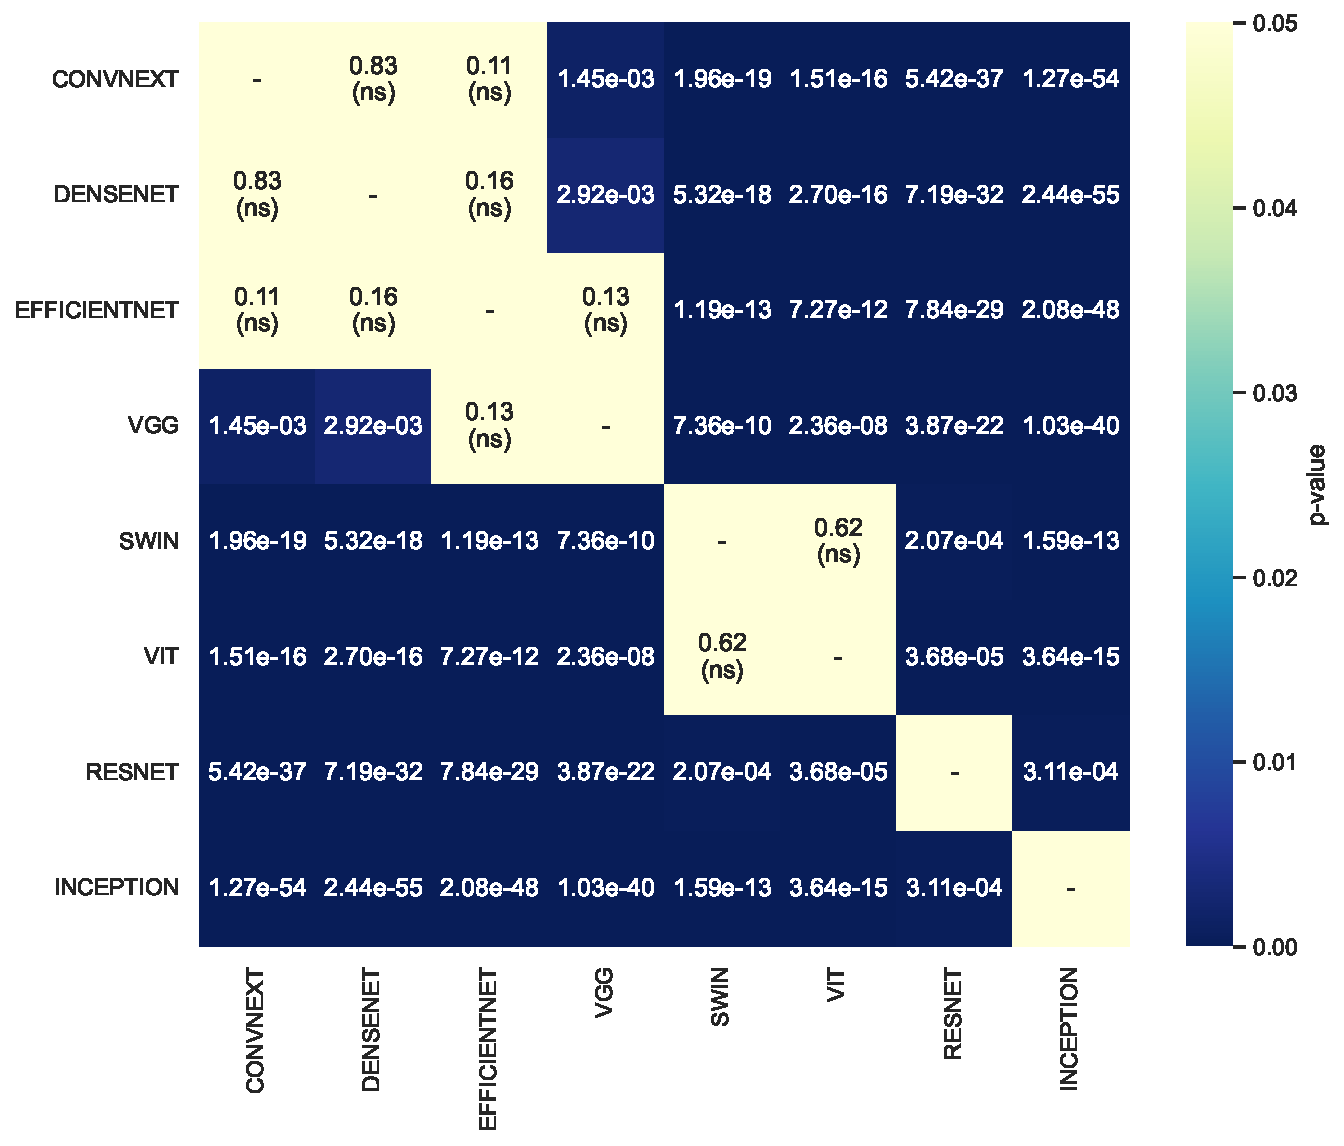
\includegraphics[width=0.8\textwidth]{images/p_value_heatmap.pdf}
  \caption{Matriz de significância estatística (McNemar) entre os modelos da versão V10.}
  \label{fig:p_value_heatmap}
\end{figure}

Observa-se que o modelo \textbf{DenseNet} apresenta uma superioridade estatisticamente robusta sobre arquiteturas como o \textit{Swin Transformer} e o \textit{ResNet}, com $p < 0,01$. Contudo, a diferença entre o DenseNet e o ConvNext, embora presente, apresenta um nível de confiança menor em certas variações, sugerindo que ambos possuem capacidades de representação similares para este domínio, apesar da DenseNet manter a liderança absoluta em MCC.
